% chapter included in forwardcom.tex
\documentclass[forwardcom.tex]{subfiles}
\begin{document}
\RaggedRight


\chapter{Numerical errors and exceptions}

\section{A different way of tracking errors}
\label{ADifferentWayOfTrackingErrors}
The two most common ways of detecting numerical errors during floating point calculations are:
\begin{enumerate}
  \item Trapping of exceptions (i.e. software interrupts)
  \item Clearing a global status register before the calculations and reading it afterwards
\end{enumerate}

These systems of error detection were designed before parallel execution were common. There is a big problem when calculations are done in parallel or out of order while the error detection systems are based on sequential logic without regard for parallel execution. Optimizations of both hardware and software are hampered by this incongruity.
\vv

SIMD code with vector registers is typically handling branches by executing both sides of a branch with the whole vector and then combining the two vector results by picking each element from one side or the other depending on a boolean vector representing the branch condition for each element. This has the consequence that a not-taken branch can cause a spurious error. Most compilers are unable to generate SIMD code for loops that contain branches unless error detection is disabled.
\vv

A further problem with trapping is that traps are supposed to occur in order. A microprocessor with out-of-order execution has to execute every instruction speculatively until it is certain that no preceding instruction will generate a trap.
\vv

The many problems with error detection during parallel execution are further discussed in the document 
\href{https://www.agner.org/optimize/nan_propagation.pdf}{www.agner.org/optimize/nan\_propagation.pdf}.
\vv

The most obvious solution to the problem of error detection in parallel systems is to use the same kind of parallelism for error detection as for program execution and to let the error information follow the same data paths as the normal calculation results.
\vv

The floating point standard (IEEE 754) defines a data type called NaN (Not a Number) that can be generated as the result of a faulty calculation. Such NaNs can propagate through a series of calculations because a calculation with a NaN input will generate an identical NaN output in most cases. This is called NaN propagation. A NaN contains a series of bits called a payload that is intended for containing diagnostic information. The payload feature is hardly ever used in common systems today, but the time has come to activate this dormant feature. The NaN propagation mechanism is further explained below on page \pageref{nanPropagation}.
\vv

ForwardCom is using NaN payloads and NaN propagation in the following way. When a calculation instruction detects a numerical error, for example overflow, then it will generate a NaN result with a payload indicating the kind of error and possibly additional diagnostic information. This NaN is contained in the same register that would contain the normal result if there was no error. 
If this register is used in further calculations, then the NaN will propagate through the series of calculations until the end result. The payload is preserved during the NaN propagation so that the cause of error can be analyzed.
\vv

This method for error detection is perfect for parallel execution. The result of a series of calculations is guaranteed to be independent of the level of parallelism because an error in one vector element will not affect the other elements of the vector.
\vv

The detection of floating point errors through NaNs can be turned on or off for each kind of error or exception by setting a control bit in the NUMCONTR register or in a mask register (see page \pageref{table:maskBits}).
\vv

While ForwardCom has no status flags, the NaN payload is replacing the 
status flags for floating point exceptions specified by the IEEE 754 standard. 
Any arithmetic operation can signal at most one exception per vector element, according to the standard.
\vv


\section{Floating point error and exception types}
\label{FloatingPointExceptionTypes}

The floating point standard (IEEE 754) defines five types of events called exceptions:

\begin{enumerate}
  \item Invalid operation, for example $0 / 0$ or sqrt$(-1)$
  \item Division by zero, when a non-zero number is divided by 0
  \item Overflow, when the result of a calculation is too big to fit the specified format
  \item Underflow, when the result of a calculation is too small to fit the specified format 
  \item Inexact, when the result of a calculation cannot fit the specified format without loss of precision  
\end{enumerate}

Each type of exception can be detected or ignored. Underflow is usually ignored and the result is set to zero. The inexact exception is also usually ignored and the result is rounded according to the specified rounding mode. 
\vv

ForwardCom includes some additional error codes that are not defined in the IEEE 754 standard. It also makes a subdivision of the exception types defined in IEEE 754. Each error or exception type has a unique binary error code that is indicated in a NaN payload.
The error and exception types and corresponding error codes are listed in table \ref{table:FPErrorTypes}.

\begin{longtable}
{|p{53mm}|p{28mm}|p{15mm}|p{26mm}|}
\caption{Floating point error and exception types}
\label{table:FPErrorTypes}
\endfirsthead
\endhead
\hline
\bfseries Error or exception & \bfseries Error code & \bfseries Control bit & \bfseries Defalt result \\ \hline

data not initialized      & \texttt{111111111} &       &  NaN \\
data not available        & \texttt{111111110} &       &  NaN \\
division by zero          & \texttt{111110111} & bit 2 & $\pm$ INF \\
division overflow         & \texttt{111101111} & bit 3 & $\pm$ INF \\
multiplication overflow   & \texttt{111101110} & bit 3 & $\pm$ INF \\
FMA overflow              & \texttt{111101101} & bit 3 & $\pm$ INF \\
add/sub overflow          & \texttt{111101100} & bit 3 & $\pm$ INF \\
conversion overflow       & \texttt{111101011} & bit 3 & $\pm$ INF \\
other overflow            & \texttt{111101010} & bit 3 & $\pm$ INF \\
$0 / 0$ invalid           & \texttt{111100111} & & NaN \\
$\infty / \infty$ invalid & \texttt{111100110} & & NaN \\
$0 * \infty$ invalid      & \texttt{111100101} & & NaN \\
$\infty - \infty$ invalid & \texttt{111100100} & & NaN \\
underflow                 & \texttt{111011111} & bit 4 & $\pm$ 0 \\
inexact                   & \texttt{111010111} & bit 5 & rounded result \\
sqrt of negative          & \texttt{111001111} &  & NaN \\
log of negative           & \texttt{111001110} &  & NaN \\
pow invalid               & \texttt{111001101} &  & NaN \\
modulo/remainder invalid  & \texttt{111001100} &  & NaN \\
asin invalid              & \texttt{111000111} &  & NaN \\
acos invalid              & \texttt{111000110} &  & NaN \\
acosh invalid             & \texttt{111000011} &  & NaN \\
atanh invalid             & \texttt{111000010} &  & NaN \\

other standard math functions  & \texttt{110xxxxxx} &  & NaN \\
other math functions      & \texttt{101xxxxxx} &  & NaN \\
other functions           & \texttt{100xxxxxx} &  & NaN \\
user-defined  & \texttt{0xxxxxxxx} &  & NaN \\
\hline
\end{longtable}
\vv

An error or exception code is inserted into a NaN as illustrated here:
\vv

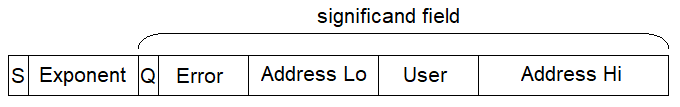
\includegraphics[width=450pt]{nan_code.png}
\vv

The field that holds the significand for normal numbers is divided into the fields Q, Error, Address low, User, and Address high for a NaN that is used as a ForwardCom error code. The fields of a NaN are used as follows:

\begin{longtable}
{|p{25mm}|p{15mm}|p{100mm}|}
\caption{NaN error codes}
\label{table:NaNErrorCode}
\endfirsthead
\endhead
\hline
\bfseries Field & \bfseries Bits & \bfseries Meaning \\ \hline
S    & 1 & Sign bit, has no meaning in NaNs \\
\hline
Exponent & 5-11 & Exponent, all ones. Size depends on precision \\
\hline
Q    & 1 & Quiet bit \\
\hline
Error code & 9 & Error or exception code from table \ref{table:FPErrorTypes} \\
\hline
Address low & 13 & Low part of code address where exception happened \\
\hline
User    & 10 & Available for user defined purposes \\
\hline
Address high & 19 & High part of code address where exception happened \\
\hline
\end{longtable}
\vv

The most important bits of the NaN payload are placed at the leftmost (most significant) positions so that they are available in low precision formats.
The half precision format (float16) has a significand of ten bits. This can contain only the Q and Error code fields. The single precision format (float32) has 23 bits in the significand. This can contain the Q, Error code, and Address low fields. The double precision format (float64) has a significand of 52 bits. This, and higher precision formats, contain the Q, Error code, Address low, User, and Address high fields. The optional format bfloat16 has a significand of only 7 bits. This can contain the Q field and the six most significant bits of the Error field. This is enough for specifying the main error or exception type, but not the subtype.
\vv

The Address low field, which is present in the single precision format, contains the lower 13 bits of the word address of the code instruction that generated the exception. 13 bits can address 32 kB of code when each code word is four bytes. If there is more than 32 kB of code, then the 13 bits cannot uniquely identify a single instruction. A debugger may help finding the source of the error by excluding addresses that do not mark the beginning of an instruction that is capable of generating an exception of the indicated type and subtype. The double precision format can hold a code address of 13+19 = 32 bits which can cover 16 GB of code. The Address high field may be made smaller if more bits are needed for the User field.
\vv

The Quiet bit (Q) is always 1 to indicate a quiet NaN when the NaN is used as an error or exception code. A NaN with Q = 0 is a signalling NaN. Signalling NaNs are used in ForwardCom only for NaN-boxing of non-numerical data, such as text strings, in programming languages with dynamic typing of variables.
\vv

Numerical exceptions such as overflow, underflow, division by zero, and inexact can be enabled or disabled by the control bits indicated in table \ref{table:FPErrorTypes}. The control bits can be set using the NUMCONTR register or a mask register.
The control bits have full granularity when a mask register is used. This means that it is possible to enable a particular exception in one vector element and disable it in another element of the same vector register by setting the control bits of a mask register accordingly. This makes it possible to do the same calculation with different settings simultaneously.
\vv

The 'data not initialized' code indicates a programming error when attempting to read data that have not been initialized. If an uninitialized range of memory is set to all 1-bits, then we will get the 'data not initialized' error when this is read as floating point data, regardless of the specified precision. Signalling NaNs are not used for this purpose.
\vv

The 'data not available' code is not the result of a calculation. It is intended to indicate that input data are not available.
\vv

These NaN codes are useful for identifying errors and exceptions. Debuggers will show the error or exception type when a NaN is displayed. Standard print functions may do the same. For example, when printing out the result of a series of calculations that involved an overflow, the result may show as "NaN(multiplication overflow)".
\vv


\section{Propagation of NaNs}
\label{nanPropagation}

Most floating point operations are sure to propagate NaNs. An instruction with a NaN input will generate a NaN output with the same payload. However, we must be aware of cases where the propagation of NaNs may fail. 
\vv

The 2019 version of the IEEE 754 standard has been corrected to make sure that the max and min functions propagate NaNs, which was not the case in previous versions. Unfortunately, a few cases remain where NaNs are not sure to propagate. Most importantly, the pow function fails to propagate a NaN in the special cases pow(NaN,0) = 1 and pow(1,NaN) = 1. ForwardCom deviates from the standard here and makes sure that pow and similar functions propagate NaNs in all cases.
\vv

Obviously, NaNs cannot propagate when floating point values are converted to integers or booleans. It is the responsibility of the programmer to check for NaNs before any such conversion or making sure the conversion instruction generates an appropriate value in case of NaN inputs. Floating point compare instructions and branch instructions are treating cases with NaN inputs as unordered. These instructions can be adjusted to treat unordered cases as either true of false (see page \pageref{table:conditionCodesForCompareInstruction} and \pageref{table:floatCompareJumpInstructions}).
\vv

Propagation of NaN payloads is rarely used in traditional systems and the current standard is not very specific about this topic. When two NaNs with different payloads are combined, i.e. NaN1 + NaN2, then one of the two payloads is propagated, but the standard does not specify which one. Current microprocessors propagate only the first NaN operand. This can lead to unpredictable behaviour since the compiler is allowed to swap the two operands. ForwardCom solves this ambiguity by propagating the highest of the payloads (interpreted as fractions while ignoring the sign bit and exponent).
\vv

Another uncertainty is that the current standard does not specify how a NaN payload is treated when converting floating point data to a different precision. A test on several common platforms has shown that the payload is left-justified during conversion. This means that the most significant bits of the payload are preserved  when converting a NaN to a lower precision. The payload is padded with trailing zeroes when converting a NaN to a higher precision. This corresponds to the way the fraction bits are treated when converting a normal number, except that the payload is not rounded when converting to a lower precision. ForwardCom follows this undocumented de facto standard. (This observation applies to computers with binary floating point formats. Computers with decimal floating point formats are right-justifying the payload, but this does not affect ForwardCom which does not support decimal floating point formats).
\vv

We have placed the most important information in the most significant bits of the NaN payload because these bits are sure to be preserved when converting to a different precision. The quiet bit is the most significant bit. The error code is left-justified next to the quiet bit so that all floating point precisions can contain an error or exception code.
\vv

The sign bit of a NaN has no meaning. Whether the sign bit of a NaN is set or cleared by a particular operation is implementation-dependent. The sign bit may change during the propagation of a NaN. The sign bit may not be shown when printing out a NaN result.
\vv


\section{Detecting integer overflow} 
\label{integerOverflowDetection}
There is no common standard method for detecting overflow in integer calculations. The detection of overflow in signed integer operations is a real nightmare in some programming languages like C++ (see 
\href{https://stackoverflow.com/questions/3944505/detecting-signed-overflow-in-c-c}{stackoverflow.com/questions/3944505/detecting-signed-overflow-in-c-c}).
\vv

Possible solutions with a status register or fault trapping are not recommended in ForwardCom for the same reasons as explained above for floating point errors. 
Instead, the following methods may be used for detecting signed and unsigned integer overflow: 

\begin{itemize}
  \item Use conditional jump instructions. \\
    Signed: add/jump\_overfl, sub/jump\_overfl. \\
    Unsigned: add/jump\_carry, sub/jump\_borrow. \\
    Division: compare with zero and jump if equal before dividing. \\
    This method cannot detect multiplication overflow.  
  
  \item Use instructions with overflow check in a vector register. 
    The even-numbered vector elements are used for calculations, while
    the odd-numbered vector elements are used for propagating error flags. 
    See page \pageref{table:addOcInstruction} for details. 
    
  \item Use floating point instructions with integer data. 
    Enable the mask bits for detection of overflow and inexact.
  
\end{itemize}
\vv

Other methods for generating error messages in function libraries are discussed on page \pageref{errorMessageHandling}.
\vv


\end{document}
